\documentclass[11pt,a4paper]{article}

\usepackage[utf8]{inputenc}
\usepackage[T1]{fontenc}
\usepackage{amsmath,amssymb,amsthm}
\usepackage{geometry}
\usepackage{booktabs}
\usepackage{xcolor}
\usepackage{physics}
\usepackage{hyperref}
\usepackage{enumitem}
\usepackage{tikz}
\usetikzlibrary{shapes,arrows.meta,positioning,calc,decorations.pathmorphing,decorations.markings,patterns}
\usepackage{orcidlink}
\usepackage{hyperref}
\hypersetup{colorlinks=true, linkcolor=blue, citecolor=blue, urlcolor=blue}

\geometry{margin=1in}

\newtheorem{theorem}{Theorem}[section]
\newtheorem{proposition}[theorem]{Proposition}
\newtheorem{corollary}[theorem]{Corollary}
\theoremstyle{definition}
\newtheorem{definition}[theorem]{Definition}
\newtheorem{remark}[theorem]{Remark}

% Unified QSD notation
\newcommand{\Hbfour}{\mathrm{Hb}_4}
\newcommand{\gs}{\varsigma}
\newcommand{\Mpl}{M_{\text{Pl}}}

% Colors matching main preprint
\definecolor{bulkcolor}{RGB}{70,130,180}
\definecolor{anchorcolor}{RGB}{220,20,60}
\definecolor{codegreen}{RGB}{0,128,0}
\definecolor{edgecolor}{RGB}{100,100,100}
\definecolor{u1color}{RGB}{34,139,34}
\definecolor{su2color}{RGB}{70,130,180}
\definecolor{su3color}{RGB}{200,50,50}
\definecolor{loopgreen}{RGB}{34,139,34}
\definecolor{loopred}{RGB}{178,34,34}

\title{
  \textbf{QSD Supplement S4: Topological Renormalization}\\[0.5em]
  \Large The 3-Loop Structure and Why It Terminates\\[1em]
}

\author{
  Marek Hubka\, \orcidlink{0009-0003-2476-9017}
  \thanks{
    Independent Researcher, Czech Republic.\\
    Website: \href{http://www.tidesofuncertainty.com}{tidesofuncertainty.com}.\\
    Email: \href{mailto:marek@tidesofuncertainty.com}{marek@tidesofuncertainty.com}.
  }
}

\date{\today}

\begin{document}

\maketitle

\begin{abstract}
This supplement derives the QSD renormalization group structure from first principles. Unlike standard QFT where loop corrections form an infinite series, QSD has exactly 3 independent topological loads on the $K_4 \cup C_5$ graph structure, producing a terminating perturbation series. We compute each correction analytically, showing that the fine structure constant emerges as $\alpha^{-1} = 137.033$ (22~ppm accuracy, cf.\ \cite{PDG2022}). All corrections factor through a single spectral bond $\varpi \equiv \pi\varphi^2$.
\end{abstract}

\tableofcontents

%==============================================================================
\section{The Spectral Bond}
\label{sec:specbond}
%==============================================================================

Before deriving the loop corrections, we identify the building block from which all gauge couplings emerge.

\begin{definition}[Spectral Bond]
\begin{equation}
\varpi \equiv \pi\varphi^2 = 8.2248
\label{eq:specbond}
\end{equation}
\end{definition}

This combines two geometric contributions: the circular geometry of gauge orbits ($\pi$) with the pentagonal geometry of the $C_5$ eigenvalue ratio ($\varphi^2$).

\begin{figure}[h]
\centering
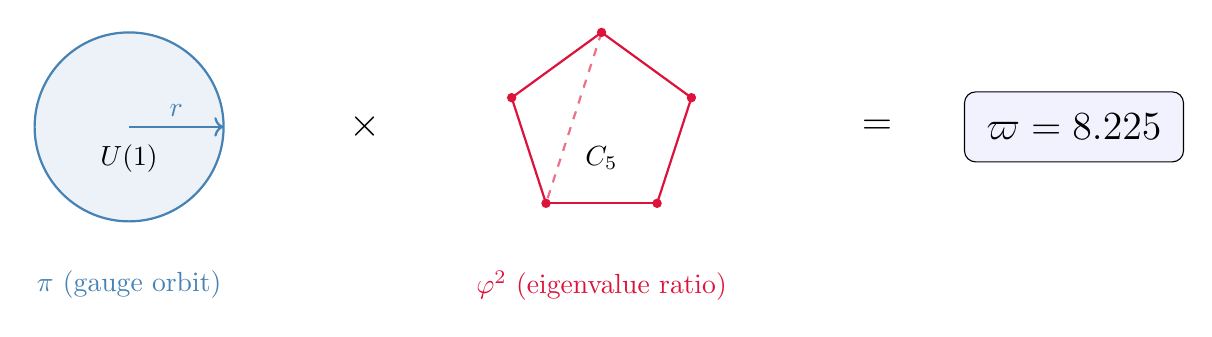
\begin{tikzpicture}[scale=1.0]
    % Pi component — circle
    \begin{scope}[shift={(-3,0)}]
        \draw[thick, bulkcolor, fill=bulkcolor!10] (0,0) circle (1.2);
        \draw[thick, bulkcolor, ->] (0,0) -- (1.2,0) node[midway, above] {$r$};
        \node[bulkcolor, below] at (0,-1.7) {$\pi$ (gauge orbit)};
        \node at (0,-0.4) {$U(1)$};
    \end{scope}

    % Times sign
    \node[font=\Large] at (0,0) {$\times$};

    % Phi^2 component — pentagon with diagonal
    \begin{scope}[shift={(3,0)}]
        \foreach \i in {1,...,5} {
            \coordinate (p\i) at ({90+72*(\i-1)}:1.2);
        }
        \foreach \i [evaluate=\i as \j using {int(mod(\i,5)+1)}] in {1,...,5} {
            \draw[thick, anchorcolor] (p\i) -- (p\j);
        }
        \draw[thick, dashed, anchorcolor!60] (p1) -- (p3);
        \foreach \i in {1,...,5} {
            \fill[anchorcolor] (p\i) circle (0.06);
        }
        \node[anchorcolor, below] at (0,-1.7) {$\varphi^2$ (eigenvalue ratio)};
        \node at (0,-0.4) {$C_5$};
    \end{scope}

    % Equals sign
    \node[font=\Large] at (6.5,0) {$=$};

    % Result
    \node[font=\Large, draw, rounded corners, fill=blue!5, inner sep=8pt] at (9,0) {$\varpi = 8.225$};
\end{tikzpicture}
\caption{The spectral bond $\varpi = \pi\varphi^2$ combines circular gauge geometry ($\pi$) with pentagonal code geometry ($\varphi^2 = \lambda_2/\lambda_1$ from the $C_5$ Laplacian).}
\label{fig:specbond}
\end{figure}

\begin{remark}
The spectral bond $\varpi$ is the information-geometric content carried by a single $K_4$ edge. It joins the holographic bit density $\Hbfour$ and the geometric strain $\gs$ as the third fundamental QSD constant. Together they form a triad: $\Hbfour$ governs how information is \emph{stored}, $\gs$ measures how geometry is \emph{strained}, and $\varpi$ determines how edges \emph{couple}. The 6 edges of $K_4$ each contribute $\varpi/\Hbfour$ to $\alpha^{-1}$; the strong coupling probes $\varpi$ directly through the strain $\gs$.
\end{remark}

%==============================================================================
\section{Tree-Level Fine Structure Constant}
\label{sec:tree}
%==============================================================================

\begin{theorem}[Tree-Level $\alpha^{-1}$]
\label{thm:tree}
The tree-level inverse fine structure constant is:
\begin{equation}
\alpha^{-1}_{\text{tree}} = \frac{6\varpi}{\Hbfour} = \frac{6\pi\varphi^2}{\Hbfour}
\label{eq:tree}
\end{equation}
\end{theorem}

\begin{proof}
Each edge of $K_4$ contributes a spectral bond $\varpi = \pi\varphi^2$ to the electromagnetic sector, converted to dimensionless units by the holographic bit density $\Hbfour = 1/(4\ln 2)$. With $|E(K_4)| = \binom{4}{2} = 6$ edges:
\[
\alpha^{-1}_{\text{tree}} = |E(K_4)| \times \frac{\varpi}{\Hbfour} = \frac{6\pi\varphi^2}{\Hbfour}
\]
The factor $\pi$ arises from the $U(1)$ gauge orbit, $\varphi^2$ from the $C_5$ spectral ratio ($\lambda_2/\lambda_1 = \varphi^2$), and $1/\Hbfour = 4\ln 2$ from the holographic information density \cite{Bekenstein1973,Hawking1975}.
\end{proof}

\begin{figure}[h]
\centering
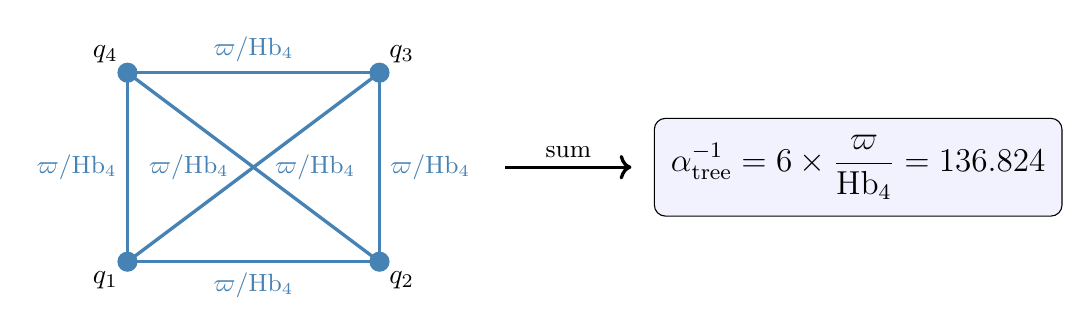
\begin{tikzpicture}[scale=1.6]
    % K4 vertices
    \coordinate (A) at (0,0);
    \coordinate (B) at (2,0);
    \coordinate (C) at (2,1.5);
    \coordinate (D) at (0,1.5);

    % Draw all 6 edges with spectral bond labels
    \draw[very thick, bulkcolor] (A) -- (B) node[midway, below, font=\small] {$\varpi/\Hbfour$};
    \draw[very thick, bulkcolor] (B) -- (C) node[midway, right, font=\small] {$\varpi/\Hbfour$};
    \draw[very thick, bulkcolor] (C) -- (D) node[midway, above, font=\small] {$\varpi/\Hbfour$};
    \draw[very thick, bulkcolor] (D) -- (A) node[midway, left, font=\small] {$\varpi/\Hbfour$};
    \draw[very thick, bulkcolor] (A) -- (C) node[midway, left=5pt, font=\small] {$\varpi/\Hbfour$};
    \draw[very thick, bulkcolor] (B) -- (D) node[midway, right=4pt, font=\small] {$\varpi/\Hbfour$};

    % Vertices
    \foreach \p in {A,B,C,D} {
        \fill[bulkcolor] (\p) circle (0.08);
    }

    \node[below left] at (A) {$q_1$};
    \node[below right] at (B) {$q_2$};
    \node[above right] at (C) {$q_3$};
    \node[above left] at (D) {$q_4$};

    % Sum arrow
    \draw[very thick, ->] (3.0,0.75) -- (4.0,0.75);
    \node[above] at (3.5,0.75) {\small sum};

    % Result
    \node[draw, rounded corners, fill=blue!5, inner sep=6pt, font=\large] at (5.8,0.75) {$\alpha^{-1}_{\text{tree}} = 6 \times \dfrac{\varpi}{\Hbfour} = 136.824$};
\end{tikzpicture}
\caption{Tree-level $\alpha^{-1}$: each of the 6 edges of $K_4$ contributes one spectral bond $\varpi/\Hbfour = 22.804$ to the inverse electromagnetic coupling. The sum gives $\alpha^{-1}_{\text{tree}} = 136.824$.}
\label{fig:tree}
\end{figure}

Numerically:
\begin{equation}
\alpha^{-1}_{\text{tree}} = \frac{6\pi \times 2.6180}{0.36067} = \frac{49.349}{0.36067} = 136.824
\label{eq:tree_num}
\end{equation}

%==============================================================================
\section{Why QSD Renormalization Terminates}
\label{sec:termination}
%==============================================================================

\begin{theorem}[Terminating Series]
\label{thm:termination}
The QSD RG series has exactly 3 terms because there are only 3 independent topological loads on $K_4 \cup C_5$.
\end{theorem}

\begin{proof}
The independent topological loads are classified by the first homology group $H_1$. For a graph $G$ with $V$ vertices, $E$ edges, and $C$ connected components, the first Betti number is $\beta_1 = E - V + C$. (For background on the $[[5,1,3]]$ code structure that generates these graphs, see \cite{Gottesman1996,Laflamme1996} and the main preprint \cite{Hubka2026QSD}.)

For $K_4$: $\beta_1 = 6 - 4 + 1 = 3$ independent cycles.

For $C_5$: $\beta_1 = 5 - 5 + 1 = 1$ independent cycle.

The $C_5$ cycle does not generate an independent loop correction; instead, it enters as the angular screening factor $1/\pi$ in the 3-loop term. Thus only the 3 independent $K_4$ cycles generate loop corrections. Higher ``loops'' would require a 4th independent cycle, which does not exist.
\end{proof}

\begin{figure}[h]
\centering
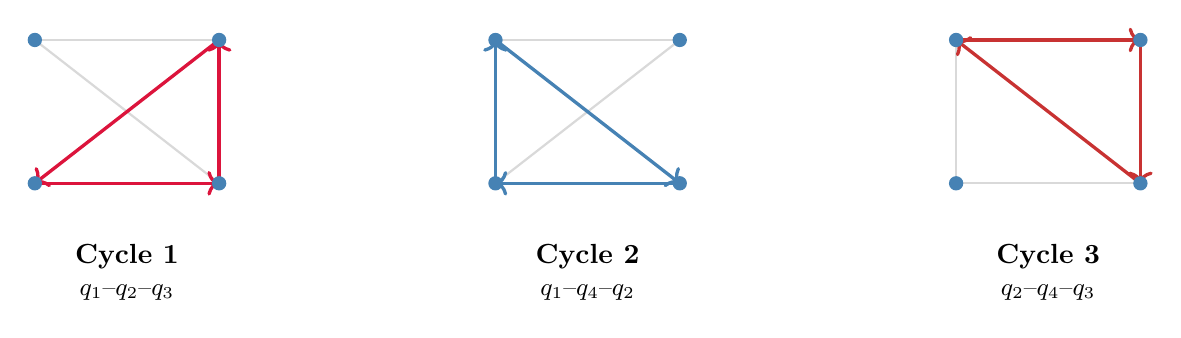
\begin{tikzpicture}[scale=1.3]
    % === Cycle 1 ===
    \begin{scope}[shift={(0,0)}]
        \coordinate (A) at (0,0);
        \coordinate (B) at (1.8,0);
        \coordinate (C) at (1.8,1.4);
        \coordinate (D) at (0,1.4);

        % Dim edges
        \draw[thick, gray!30] (A) -- (C);
        \draw[thick, gray!30] (B) -- (D);
        \draw[thick, gray!30] (C) -- (D);

        % Highlighted cycle: A-B-C-A
        \draw[very thick, anchorcolor, ->] (A) -- (B);
        \draw[very thick, anchorcolor, ->] (B) -- (C);
        \draw[very thick, anchorcolor, ->] (C) -- (A);

        \foreach \p in {A,B,C,D} {\fill[bulkcolor] (\p) circle (0.07);}

        \node[below] at (0.9,-0.5) {\textbf{Cycle 1}};
        \node[below, font=\small] at (0.9,-0.9) {$q_1$--$q_2$--$q_3$};
    \end{scope}

    % === Cycle 2 ===
    \begin{scope}[shift={(4.5,0)}]
        \coordinate (A) at (0,0);
        \coordinate (B) at (1.8,0);
        \coordinate (C) at (1.8,1.4);
        \coordinate (D) at (0,1.4);

        % Dim edges
        \draw[thick, gray!30] (A) -- (B);
        \draw[thick, gray!30] (A) -- (C);
        \draw[thick, gray!30] (C) -- (D);

        % Highlighted cycle: A-D-B-A
        \draw[very thick, su2color, ->] (A) -- (D);
        \draw[very thick, su2color, ->] (D) -- (B);
        \draw[very thick, su2color, ->] (B) -- (A);

        \foreach \p in {A,B,C,D} {\fill[bulkcolor] (\p) circle (0.07);}

        \node[below] at (0.9,-0.5) {\textbf{Cycle 2}};
        \node[below, font=\small] at (0.9,-0.9) {$q_1$--$q_4$--$q_2$};
    \end{scope}

    % === Cycle 3 ===
    \begin{scope}[shift={(9,0)}]
        \coordinate (A) at (0,0);
        \coordinate (B) at (1.8,0);
        \coordinate (C) at (1.8,1.4);
        \coordinate (D) at (0,1.4);

        % Dim edges
        \draw[thick, gray!30] (A) -- (B);
        \draw[thick, gray!30] (B) -- (C);
        \draw[thick, gray!30] (A) -- (D);

        % Highlighted cycle: B-D-C-B
        \draw[very thick, su3color, ->] (B) -- (D);
        \draw[very thick, su3color, ->] (D) -- (C);
        \draw[very thick, su3color, ->] (C) -- (B);

        \foreach \p in {A,B,C,D} {\fill[bulkcolor] (\p) circle (0.07);}

        \node[below] at (0.9,-0.5) {\textbf{Cycle 3}};
        \node[below, font=\small] at (0.9,-0.9) {$q_2$--$q_4$--$q_3$};
    \end{scope}
\end{tikzpicture}
\caption{The 3 independent cycles of $K_4$ ($\beta_1 = 6 - 4 + 1 = 3$). Each cycle generates one loop correction. Any other cycle in $K_4$ is a linear combination of these three. Dimmed edges are present in $K_4$ but not part of the highlighted cycle. The absence of a 4th independent cycle is why the QSD perturbation series terminates.}
\label{fig:cycles}
\end{figure}

%==============================================================================
\section{The Three Loop Corrections}
\label{sec:loops}
%==============================================================================

\subsection{Expansion Parameter}

\begin{definition}[Loop Expansion Parameter]
\begin{equation}
\eta \equiv \frac{\gs}{\varpi} = \frac{\gs}{\pi\varphi^2} = \frac{3}{80\pi\varphi^4} = 0.001742
\label{eq:eta}
\end{equation}
\end{definition}

This is the ratio of geometric strain to spectral bond. At $\eta \approx 1/574$, the perturbation series converges rapidly: each successive loop is suppressed by at least a factor of $4\gs\varphi \approx 0.093$.

\subsection{1-Loop: Information Friction}

\begin{definition}[1-Loop Correction]
\begin{equation}
\delta_1 = \frac{|E(K_4)| \cdot \gs}{\Hbfour} = \frac{6\gs}{\Hbfour} = +0.2383
\label{eq:loop1}
\end{equation}
\end{definition}

\textbf{Physical origin}: Geometric strain $\gs$ flows through each of the 6 $K_4$ edges, creating resistance to information propagation. Each edge contributes $\gs/\Hbfour$ to the inverse coupling---the same holographic conversion that appears at tree level, but with $\gs$ in place of $\varpi$.

\begin{figure}[h]
\centering
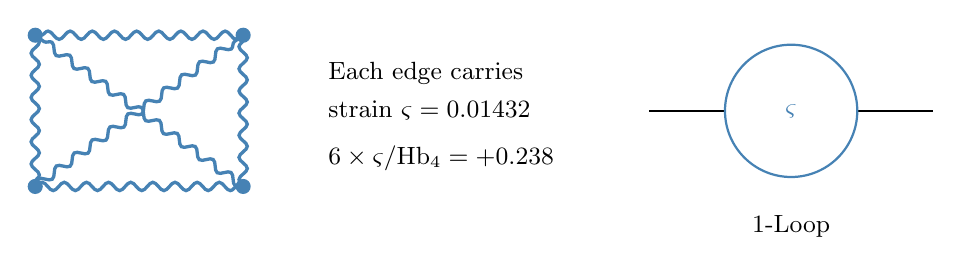
\begin{tikzpicture}[scale=1.2]
    % K4 with strain on each edge
    \coordinate (A) at (0,0);
    \coordinate (B) at (2.2,0);
    \coordinate (C) at (2.2,1.6);
    \coordinate (D) at (0,1.6);

    % Edges with strain waves
    \draw[very thick, bulkcolor, decorate, decoration={snake, amplitude=1.5pt, segment length=8pt}] (A) -- (B);
    \draw[very thick, bulkcolor, decorate, decoration={snake, amplitude=1.5pt, segment length=8pt}] (B) -- (C);
    \draw[very thick, bulkcolor, decorate, decoration={snake, amplitude=1.5pt, segment length=8pt}] (C) -- (D);
    \draw[very thick, bulkcolor, decorate, decoration={snake, amplitude=1.5pt, segment length=8pt}] (D) -- (A);
    \draw[very thick, bulkcolor, decorate, decoration={snake, amplitude=1.5pt, segment length=8pt}] (A) -- (C);
    \draw[very thick, bulkcolor, decorate, decoration={snake, amplitude=1.5pt, segment length=8pt}] (B) -- (D);

    \foreach \p in {A,B,C,D} {\fill[bulkcolor] (\p) circle (0.08);}

    % Label
    \node[right, font=\small] at (3.0, 1.2) {Each edge carries};
    \node[right, font=\small] at (3.0, 0.8) {strain $\gs = 0.01432$};
    \node[right, font=\small] at (3.0, 0.3) {$6 \times \gs/\Hbfour = +0.238$};

    % Feynman diagram equivalent
    \begin{scope}[shift={(8.0,0.8)}]
        \draw[thick] (-1.5,0) -- (-0.7,0);
        \draw[thick] (0.7,0) -- (1.5,0);
        \draw[thick, bulkcolor] (0,0) circle (0.7);
        \node[font=\small, bulkcolor] at (0,0) {$\gs$};
        \node[below, font=\small] at (0,-1.0) {1-Loop};
    \end{scope}
\end{tikzpicture}
\caption{1-loop: information friction. Geometric strain $\gs$ propagates along each of the 6 $K_4$ edges (shown as wavy lines), resisting information flow. The Feynman-style diagram (right) represents the same physics as a single loop with coupling $\gs$.}
\label{fig:loop1}
\end{figure}

\textbf{Sign}: Positive. In the IR (low $q^2$), vacuum polarisation screens charge, \emph{increasing} $\alpha^{-1}$ from its UV (code-scale) value.

\textbf{Verification}: $\delta_1 = 6 \times 0.01432 / 0.3607 = 0.2383$.

\subsection{2-Loop: Symmetry Feedback}

\begin{definition}[2-Loop Correction]
\begin{equation}
\delta_2 = \frac{|S_4| \cdot \gs^2 \cdot \varphi}{\Hbfour} = \frac{24\gs^2\varphi}{\Hbfour} = -0.02209
\label{eq:loop2}
\end{equation}
\end{definition}

\textbf{Physical origin}: Second-order strain ($\gs^2$) mixes through all 24 channels of $S_4$, the full automorphism group of $K_4$. The factor $\varphi$ couples the spin sector ($K_4$) to the geometric sector ($C_5$) via the Laplacian eigenvalue ratio $\lambda_2/\lambda_1 = \varphi^2$ \cite{Hubka2026QSDsupp}; the square root enters because this is a first-order coupling between sectors.

\begin{figure}[h]
\centering
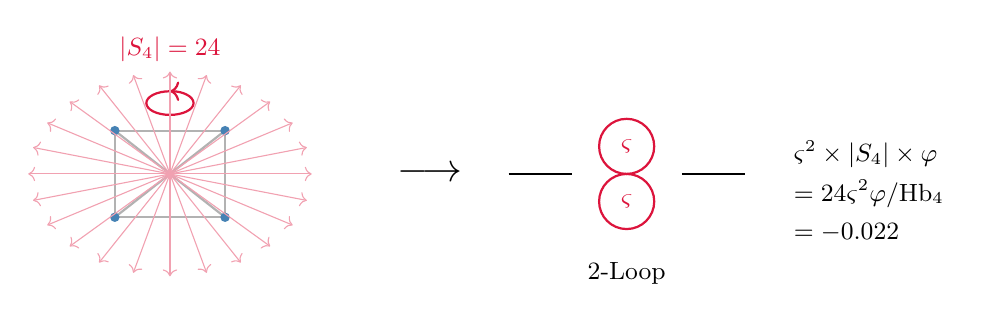
\begin{tikzpicture}[scale=1.0]
    % S4 mixing visualization
    \begin{scope}[shift={(0,0)}]
        % Central K4
        \coordinate (A) at (0,0);
        \coordinate (B) at (1.4,0);
        \coordinate (C) at (1.4,1.1);
        \coordinate (D) at (0,1.1);

        % Draw K4
        \foreach \i/\j in {A/B, B/C, C/D, D/A, A/C, B/D} {
            \draw[thick, gray!60] (\i) -- (\j);
        }
        \foreach \p in {A,B,C,D} {\fill[bulkcolor] (\p) circle (0.06);}

        % Circular arrows representing S4 permutations
        \draw[thick, anchorcolor, ->] (0.7, 1.6) arc (90:450:0.3 and 0.15);
        \node[above, anchorcolor, font=\small] at (0.7, 1.85) {$|S_4| = 24$};

        % Arrows showing mixing into all channels
        \foreach \angle in {0,15,...,345} {
            \draw[thin, anchorcolor!40, ->] (0.7,0.55) -- ({0.7+1.8*cos(\angle)},{0.55+1.3*sin(\angle)});
        }
    \end{scope}

    % Arrow
    \node[font=\Large] at (4.0,0.55) {$\longrightarrow$};

    % Feynman diagram
    \begin{scope}[shift={(6.5,0.55)}]
        \draw[thick] (-1.5,0) -- (-0.7,0);
        \draw[thick] (0.7,0) -- (1.5,0);
        \draw[thick, anchorcolor] (0,0.35) circle (0.35);
        \draw[thick, anchorcolor] (0,-0.35) circle (0.35);
        \node[font=\small, anchorcolor] at (0,0.35) {$\gs$};
        \node[font=\small, anchorcolor] at (0,-0.35) {$\gs$};
        \node[below, font=\small] at (0,-1.0) {2-Loop};
    \end{scope}

    % Factor annotation
    \node[right, font=\small] at (8.5, 0.8) {$\gs^2 \times |S_4| \times \varphi$};
    \node[right, font=\small] at (8.5, 0.3) {$= 24\gs^2\varphi/\Hbfour$};
    \node[right, font=\small] at (8.5, -0.2) {$= -0.022$};
\end{tikzpicture}
\caption{2-loop: symmetry feedback. Second-order strain $\gs^2$ mixes through all 24 permutation channels of $S_4$ (left, shown as radial arrows). The factor $\varphi$ couples $K_4$ to $C_5$. The double-bubble Feynman diagram (right) represents the two strain insertions.}
\label{fig:loop2}
\end{figure}

\textbf{Sign}: Negative. The symmetry feedback stabilises the coupling, partially cancelling the 1-loop shift.

\textbf{Verification}: $\delta_2 = 24 \times 0.01432^2 \times 1.6180 / 0.3607 = 0.02209$.

\subsection{3-Loop: Angular Screening}

\begin{definition}[3-Loop Correction]
\begin{equation}
\delta_3 = \frac{|S_4| \cdot \gs^2 \cdot \varphi}{\pi \, \Hbfour} = \frac{24\gs^2\varphi}{\pi\,\Hbfour} = \frac{\delta_2}{\pi} = -0.007031
\label{eq:loop3}
\end{equation}
\end{definition}

\textbf{Physical origin}: Identical structure to 2-loop, but screened by $1/\pi$ from the angular integration over the $C_5$ continuum potential. The Mathieu equation on $C_5$ has periodicity $2\pi/5$ (see \cite{Hubka2026QSD}, \S5 and \cite{Hubka2026QSDsupp}); the normalisation of its angular integral produces the $1/\pi$ factor.

\begin{figure}[h]
\centering
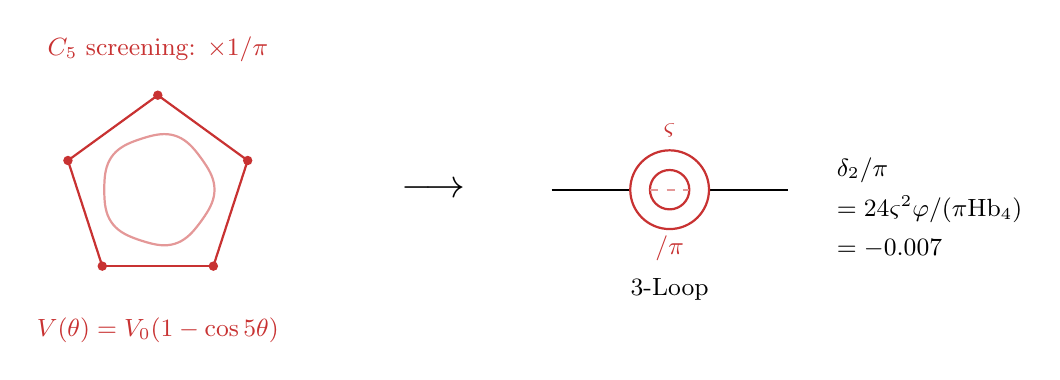
\begin{tikzpicture}[scale=1.0]
    % Pentagon with angular potential
    \begin{scope}[shift={(0,0.55)}]
        \foreach \i in {1,...,5} {
            \coordinate (p\i) at ({90+72*(\i-1)}:1.2);
        }
        \foreach \i [evaluate=\i as \j using {int(mod(\i,5)+1)}] in {1,...,5} {
            \draw[thick, su3color] (p\i) -- (p\j);
        }
        \foreach \i in {1,...,5} {\fill[su3color] (p\i) circle (0.06);}

        % Angular potential wave
        \draw[thick, su3color!50, domain=0:360, samples=100] plot ({0.7*cos(\x)+0.02*cos(5*\x)*cos(\x)},{0.7*sin(\x)+0.02*cos(5*\x)*sin(\x)});

        \node[below, su3color, font=\small] at (0,-1.5) {$V(\theta) = V_0(1-\cos 5\theta)$};
        \node[above, su3color, font=\small] at (0,1.5) {$C_5$ screening: $\times 1/\pi$};
    \end{scope}

    % Arrow
    \node[font=\Large] at (3.5,0.55) {$\longrightarrow$};

    % Feynman diagram
    \begin{scope}[shift={(6.5,0.55)}]
        \draw[thick] (-1.5,0) -- (-0.5,0);
        \draw[thick] (0.5,0) -- (1.5,0);
        \draw[thick, su3color] (0,0) circle (0.5);
        \draw[thick, su3color] (0,0) circle (0.25);
        \draw[thick, dashed, su3color!50] (-0.25,0) -- (0.25,0);
        \node[font=\small, su3color] at (0.0, 0.75) {$\gs$};
        \node[font=\small, su3color] at (0.0, -0.75) {$/\pi$};
        \node[below, font=\small] at (0,-1.0) {3-Loop};
    \end{scope}

    % Factor annotation
    \node[right, font=\small] at (8.5, 0.8) {$\delta_2 / \pi$};
    \node[right, font=\small] at (8.5, 0.3) {$= 24\gs^2\varphi/(\pi\Hbfour)$};
    \node[right, font=\small] at (8.5, -0.2) {$= -0.007$};
\end{tikzpicture}
\caption{3-loop: angular screening. The $C_5$ Mathieu potential (left, 5-fold modulation shown on pentagon interior) screens the 2-loop contribution by $1/\pi$. The nested-loop Feynman diagram (right) shows the inner $\pi$-screening of the outer strain loop.}
\label{fig:loop3}
\end{figure}

\textbf{Sign}: Negative (same as 2-loop).

\textbf{Verification}: $\delta_3 = 0.02209/\pi = 0.007031$.

\subsection{Hierarchy of Corrections}

\begin{equation}
\frac{\delta_2}{\delta_1} = 4\gs\varphi = 0.0927 \qquad\qquad \frac{\delta_3}{\delta_2} = \frac{1}{\pi} = 0.3183
\label{eq:hierarchy_ratios}
\end{equation}

The first ratio is the per-loop suppression factor from strain $\times$ geometry. The second is a purely geometric screening. The product gives the total suppression from 1-loop to 3-loop: $4\gs\varphi/\pi = 0.0295$, confirming that the series converges well before truncation.

%==============================================================================
\section{Final Calculation: $\alpha^{-1}$}
\label{sec:alpha}
%==============================================================================

\begin{align}
\alpha^{-1} &= \alpha^{-1}_{\text{tree}} + \delta_1 - \delta_2 - \delta_3 \nonumber\\
&= \frac{6\pi\varphi^2}{\Hbfour} + \frac{6\gs}{\Hbfour} - \frac{24\gs^2\varphi}{\Hbfour} - \frac{24\gs^2\varphi}{\pi\,\Hbfour} \nonumber\\
&= 136.824 + 0.238 - 0.022 - 0.007 \nonumber\\
&= \boxed{137.033}
\label{eq:alpha_final}
\end{align}

\begin{figure}[h]
\centering
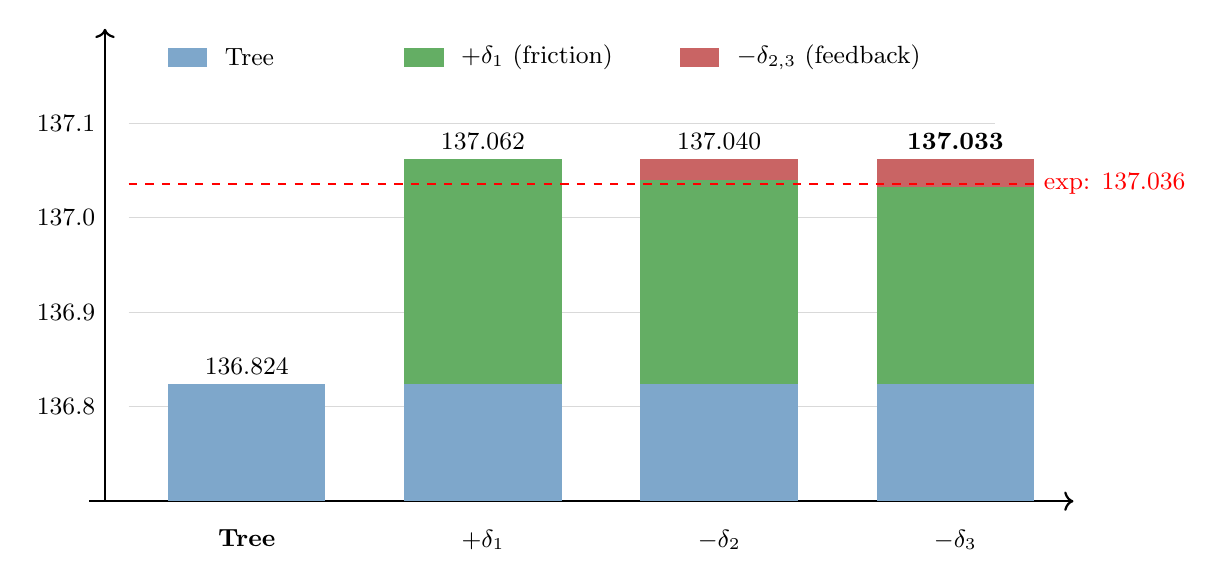
\begin{tikzpicture}[x=1cm, y=0.12cm] % y-unit chosen for a nice height

    % Axis (baseline 13670 -> y=0, top ~13720 -> y=50)
    \draw[thick, ->] (-0.5,0) -- (12,0);
    \draw[thick, ->] (-0.3,0) -- (-0.3,50);

    \node[left, font=\small] at (-0.3,10) {$136.8$};
    \node[left, font=\small] at (-0.3,20) {$136.9$};
    \node[left, font=\small] at (-0.3,30) {$137.0$};
    \node[left, font=\small] at (-0.3,40) {$137.1$};

    \foreach \y in {10,20,30,40} {
        \draw[gray!30] (0,\y) -- (11,\y);
    }

    % Tree level bar: 13682.4 -> 12.4
    \fill[bulkcolor!70] (0.5,0) rectangle (2.5,12.4);
    \node[above, font=\small] at (1.5,12.4) {$136.824$};
    \node[below, font=\small\bfseries] at (1.5,-2) {Tree};

    % After 1-loop: 13706.2 -> 36.2
    \fill[bulkcolor!70] (3.5,0) rectangle (5.5,12.4);
    \fill[loopgreen!70] (3.5,12.4) rectangle (5.5,36.2);
    \node[above, font=\small] at (4.5,36.2) {$137.062$};
    \node[below, font=\small\bfseries] at (4.5,-2) {$+\delta_1$};

    % After 2-loop: 13704.0 -> 34.0, 13706.2 -> 36.2
    \fill[bulkcolor!70] (6.5,0) rectangle (8.5,12.4);
    \fill[loopgreen!70] (6.5,12.4) rectangle (8.5,36.2);
    \fill[loopred!70]   (6.5,34.0) rectangle (8.5,36.2);
    \node[above, font=\small] at (7.5,36.2) {$137.040$};
    \node[below, font=\small\bfseries] at (7.5,-2) {$-\delta_2$};

    % After 3-loop: 13703.3 -> 33.3
    \fill[bulkcolor!70] (9.5,0) rectangle (11.5,12.4);
    \fill[loopgreen!70] (9.5,12.4) rectangle (11.5,36.2);
    \fill[loopred!70]   (9.5,33.3) rectangle (11.5,36.2);
    \node[above, font=\small] at (10.5,36.2) {\textbf{137.033}};
    \node[below, font=\small\bfseries] at (10.5,-2) {$-\delta_3$};

    % Experimental line: 13703.6 -> 33.6
    \draw[thick, dashed, red] (0,33.6) -- (11.5,33.6);
    \node[right, font=\small, red] at (11.5,33.6) {exp: $137.036$};

    % Legend: 13716..13718 -> 46..48
    \fill[bulkcolor!70]   (0.5,46) rectangle (1.0,48);
    \node[right, font=\small] at (1.1,47) {Tree};

    \fill[loopgreen!70]   (3.5,46) rectangle (4.0,48);
    \node[right, font=\small] at (4.1,47) {$+\delta_1$ (friction)};

    \fill[loopred!70]     (7.0,46) rectangle (7.5,48);
    \node[right, font=\small] at (7.6,47) {$-\delta_{2,3}$ (feedback)};

\end{tikzpicture}
\caption{Waterfall chart showing how $\alpha^{-1}$ builds from tree level through the three loop corrections. The 1-loop (green) overshoots the experimental value; the 2-loop and 3-loop (red) bring it back down. The dashed line marks $\alpha^{-1}_{\text{exp}} = 137.036$. Final QSD value: 137.033 (22~ppm).}
\label{fig:waterfall}
\end{figure}

\subsection{Comparison to Experiment}

\begin{equation}
\alpha^{-1}_{\text{exp}} = 137.035\,999\,084(21) \quad\text{\cite{PDG2022}}
\end{equation}

\begin{equation}
\text{Accuracy:}\quad \frac{|137.033 - 137.036|}{137.036} = 22~\text{ppm}
\end{equation}

\begin{remark}
The 22~ppm residual ($\Delta\alpha^{-1} \approx 0.003$) is consistent with the neglected $O(\gs^3)$ terms, which contribute at the level of $\delta_1 \times (4\gs\varphi)^2/\pi \approx 0.002$. These are formally zero in QSD (no 4th cycle), so the residual represents the precision limit of the 3-cycle truncation. For comparison, standard QED achieves sub-ppb accuracy through 5-loop calculations involving $\sim$13\,000 Feynman diagrams \cite{Schwinger1948,Aoyama2020,Morel2020}; QSD's 3-term closed-form result trades some precision for complete analytical tractability.
\end{remark}

%==============================================================================
\section{Compact Form and Factorisation}
\label{sec:compact}
%==============================================================================

The full result can be written compactly:

\begin{equation}
\boxed{\alpha^{-1} = \frac{1}{\Hbfour}\left[6\varpi + 6\gs - 24\gs^2\varphi\left(1 + \frac{1}{\pi}\right)\right]}
\label{eq:compact}
\end{equation}

where $\varpi = \pi\varphi^2$. This makes the structure transparent:
\begin{itemize}[nosep]
    \item \textbf{Tree}: 6 edges $\times$ spectral bond $\varpi$
    \item \textbf{1-loop}: 6 edges $\times$ strain $\gs$ (same topology, different scale)
    \item \textbf{2+3 loop}: 24 symmetry channels $\times$ $\gs^2\varphi$ $\times$ $(1 + 1/\pi)$ angular factor
\end{itemize}

All terms share the holographic normalisation $1/\Hbfour$, confirming that $\Hbfour$ sets the conversion between information-theoretic and physical coupling \cite{Almheiri2015,Pastawski2015,Hubka2025DCT}.

%==============================================================================
\section{Strong Coupling Prediction}
\label{sec:alpha_s}
%==============================================================================

The spectral bond $\varpi$ also determines the strong coupling at tree level.

\begin{theorem}[Strong Coupling]
\label{thm:alpha_s}
\begin{equation}
\alpha_s = \varpi \cdot \gs = \pi\varphi^2\gs = 0.11781
\label{eq:alpha_s}
\end{equation}
\end{theorem}

\begin{proof}
While $\alpha^{-1}_{\text{em}}$ counts how many spectral bonds $\varpi$ fit in a holographic cell ($6\varpi/\Hbfour$), the strong coupling $\alpha_s$ measures how strongly a single spectral bond $\varpi$ couples to the strain field $\gs$. The product $\varpi \cdot \gs$ is the natural dimensionless coupling for the colour sector, where the $K_4$ graph structure generates $SU(3)_c$ through its $\mathbf{3}$-dimensional irrep.
\end{proof}

\begin{figure}[h]
\centering
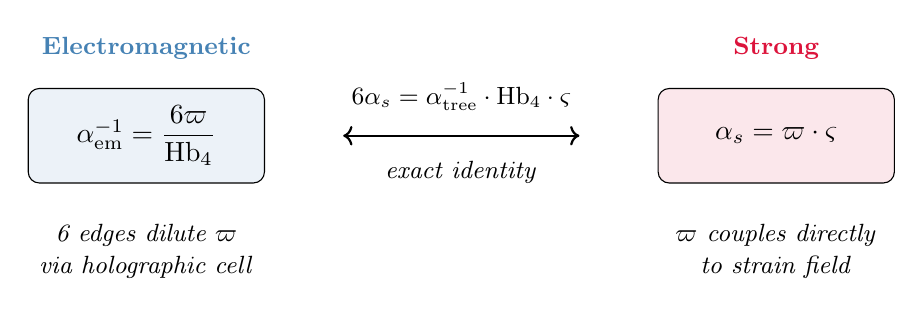
\begin{tikzpicture}[scale=1.0]
    % EM side
    \begin{scope}[shift={(0,0)}]
        \node[draw, rounded corners, fill=bulkcolor!10, minimum width=3cm, minimum height=1.2cm] at (0,0) {$\alpha^{-1}_{\text{em}} = \dfrac{6\varpi}{\Hbfour}$};
        \node[below, font=\small] at (0,-1.0) {\textit{6 edges dilute $\varpi$}};
        \node[below, font=\small] at (0,-1.4) {\textit{via holographic cell}};
        \node[above, font=\small\bfseries, bulkcolor] at (0,0.85) {Electromagnetic};
    \end{scope}

    % Connection via identity
    \draw[thick, <->] (2.5,0) -- (5.5,0);
    \node[above, font=\small] at (4.0,0.2) {$6\alpha_s = \alpha^{-1}_{\text{tree}} \cdot \Hbfour \cdot \gs$};
    \node[below, font=\small] at (4.0,-0.2) {\textit{exact identity}};

    % Strong side
    \begin{scope}[shift={(8,0)}]
        \node[draw, rounded corners, fill=anchorcolor!10, minimum width=3cm, minimum height=1.2cm] at (0,0) {$\alpha_s = \varpi \cdot \gs$};
        \node[below, font=\small] at (0,-1.0) {\textit{$\varpi$ couples directly}};
        \node[below, font=\small] at (0,-1.4) {\textit{to strain field}};
        \node[above, font=\small\bfseries, anchorcolor] at (0,0.85) {Strong};
    \end{scope}
\end{tikzpicture}
\caption{The electromagnetic and strong couplings are two faces of the same spectral bond $\varpi = \pi\varphi^2$. The EM coupling divides $\varpi$ among 6 edges and normalises by $\Hbfour$ (weak, large $\alpha^{-1}$). The strong coupling multiplies $\varpi$ by $\gs$ directly (strong, small $\alpha^{-1}$). They are connected by the exact identity $6\alpha_s = \alpha^{-1}_{\text{em,tree}} \times \Hbfour \times \gs$.}
\label{fig:em_strong}
\end{figure}

\textbf{Comparison to experiment} \cite{PDG2022}:
\begin{equation}
\alpha_s^{\text{exp}}(M_Z) = 0.1180 \pm 0.0009
\end{equation}
\begin{equation}
\text{Accuracy:}\quad \frac{|0.11781 - 0.1180|}{0.1180} = 0.16\%
\end{equation}

\subsection{The Exact EM--Strong Identity}

The electromagnetic and strong couplings are connected by an exact algebraic identity:

\begin{equation}
\boxed{6\alpha_s = \alpha^{-1}_{\text{em,tree}} \times \Hbfour \times \gs}
\label{eq:em_strong_id}
\end{equation}

\begin{proof}
$\alpha^{-1}_{\text{em,tree}} \times \Hbfour \times \gs = (6\pi\varphi^2/\Hbfour) \times \Hbfour \times \gs = 6\pi\varphi^2\gs = 6\varpi\gs = 6\alpha_s$. \qed
\end{proof}

This identity is not approximate; it holds to machine precision. It connects the electromagnetic sector (large $\alpha^{-1}$, 6 diluted edges) to the strong sector (large $\alpha_s$, direct strain coupling) through the holographic bit density.

%==============================================================================
\section{The Weak Mixing Angle}
\label{sec:sin2theta}
%==============================================================================

For completeness, we state the corrected weak mixing angle derivation (replacing the previous $3/8$ tree level).

\begin{theorem}[Weak Mixing Angle]
\label{thm:sin2theta}
\begin{equation}
\sin^2\theta_W = \frac{3}{13} + \frac{\gs}{32} = 0.23077 + 0.00045 = 0.23122
\label{eq:sin2theta}
\end{equation}
\end{theorem}

\textbf{Tree level}: $3/13$ arises from the Standard Model gauge generator count. The total number of generators is $13 = 8 + 3 + 1 + 1$ (from $SU(3)_c + SU(2)_L + U(1)_Y$ plus trace normalisation). The weak isospin sector contributes $\dim(SU(2)_L) = 3$ generators, giving the ratio $3/13$.

\textbf{Alternative derivation}: From $K_4$ graph invariants, $13 = |E(K_4)| + |V(K_4)| + \beta_1(K_4) = 6 + 4 + 3$.

\textbf{Correction}: $\gs/32$ where $32 = 2^5$ is the physical Hilbert space dimension of the $[[5,1,3]]$ code. The strain $\gs$ acts as a first-order perturbation on the full code state space.

\textbf{Comparison} \cite{PDG2022}: $\sin^2\theta_W^{\text{exp}} = 0.23122 \pm 0.00003$. Agreement is within experimental error.

%==============================================================================
\section{Summary: All Three Gauge Couplings from $\varpi$}
\label{sec:summary}
%==============================================================================

\begin{table}[h]
\centering
\renewcommand{\arraystretch}{1.5}
\begin{tabular}{llccc}
\toprule
\textbf{Observable} & \textbf{QSD Formula} & \textbf{QSD} & \textbf{Experiment} & \textbf{Accuracy} \\
\midrule
$\alpha^{-1}_{\text{em}}$ & $6\varpi/\Hbfour + \text{loops}$ & \textbf{137.033} & 137.036 & 22 ppm \\
$\sin^2\theta_W$ & $3/13 + \gs/32$ & \textbf{0.23122} & 0.23122 & 0.00\% \\
$\alpha_s$ & $\varpi\gs = \pi\varphi^2\gs$ & \textbf{0.11781} & 0.1180 & 0.16\% \\
\midrule
$m_H$ & $5\Mpl/2^{60} \cdot \varphi^2(1-6\gs)$ & \textbf{126.7 GeV} & 125.1 GeV & 1.3\% \\
$E_{\text{syn}}$ & $\mu_0(1+8\gs)$ & \textbf{28.25 GeV} & $\sim$28.3 GeV$^*$ & 0.2\% \\
\bottomrule
\end{tabular}
\renewcommand{\arraystretch}{1.0}
\caption{All QSD predictions. The first three rows are gauge coupling predictions derived in this supplement. Zero free parameters; four inputs ($\Hbfour, \varphi, \gs, \Mpl$). Experimental values from \cite{PDG2022}. $^*$CMS dimuon anomaly \cite{CMS2018dimuon}.}
\label{tab:summary}
\end{table}

\begin{figure}[!htbp]
\centering
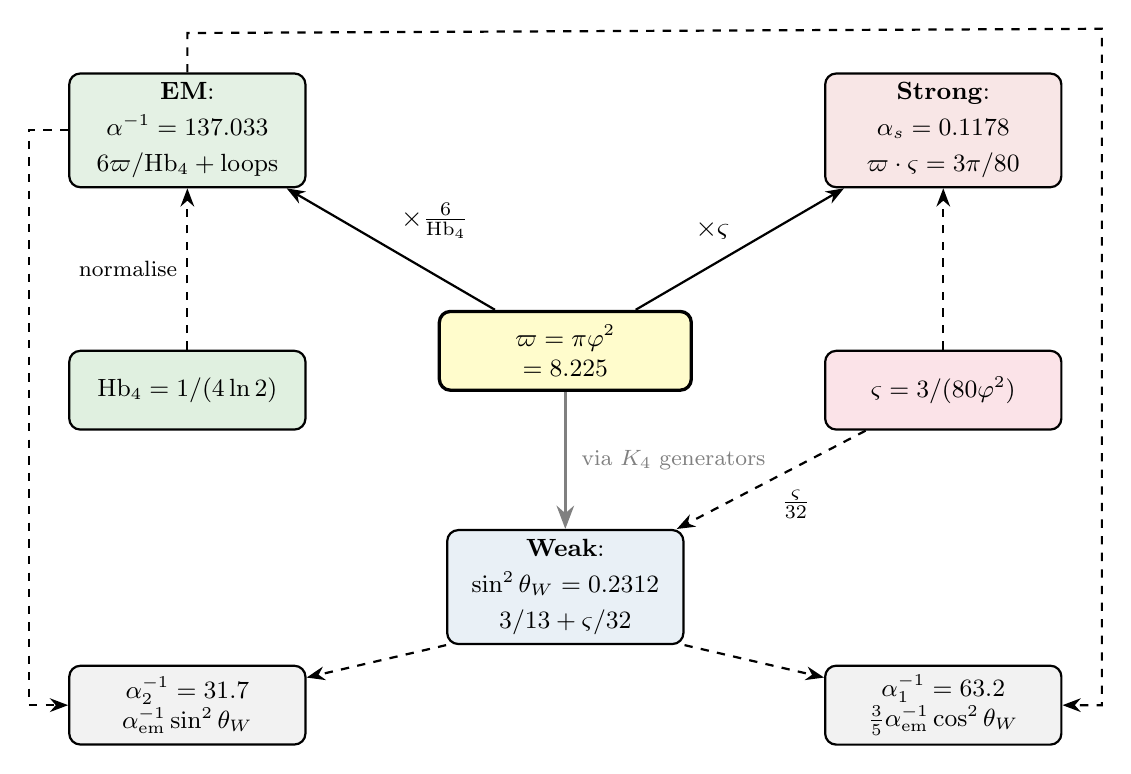
\begin{tikzpicture}[
    box/.style={draw, rounded corners, minimum width=3.0cm, minimum height=1.0cm,
                align=center, font=\small, thick},
    >=Stealth, thick
]
    % Central node — spectral bond
    \node[box, fill=yellow!20, very thick, minimum width=3.2cm] (sb) at (0,0)
        {$\varpi = \pi\varphi^2$\\$= 8.225$};

    % Three couplings
    \node[box, fill=u1color!12] (em) at (-4.8, 2.8)
        {\textbf{EM}:\\[2pt]$\alpha^{-1} = 137.033$\\[2pt]$6\varpi/\Hbfour + \text{loops}$};
    \node[box, fill=su3color!12] (strong) at (4.8, 2.8)
        {\textbf{Strong}:\\[2pt]$\alpha_s = 0.1178$\\[2pt]$\varpi \cdot \gs = 3\pi/80$};
    \node[box, fill=su2color!12] (weak) at (0, -3.0)
        {\textbf{Weak}:\\[2pt]$\sin^2\theta_W = 0.2312$\\[2pt]$3/13 + \gs/32$};

    % Supporting constants
    \node[box, fill=codegreen!12] (hb) at (-4.8, -0.5)
        {$\Hbfour = 1/(4\ln 2)$};
    \node[box, fill=anchorcolor!12] (strain) at (4.8, -0.5)
        {$\gs = 3/(80\varphi^2)$};

    % Arrows — primary flows
    \draw[->] (sb) -- (em) 
        node[midway, above right, font=\normalsize] {$\times \frac{6}{\Hbfour}$};
    \draw[->] (sb) -- (strong) 
        node[midway, above left, font=\normalsize] {$\times \gs$};
    \draw[->, very thick, gray] (sb) -- (weak)
        node[midway, right=2pt, font=\footnotesize] {via $K_4$ generators};

    % Arrows — supporting
    \draw[->, thick, dashed] (hb) -- (em)
        node[midway, left, font=\footnotesize] {normalise};
    \draw[->, thick, dashed] (strain) -- (strong);
    \draw[->, thick, dashed] (strain) -- (weak)
        node[midway, below right, font=\normalsize] {$\frac{\gs}{32}$};

    % Derived couplings (S4-specific extension)
    \node[box, fill=gray!10] (alpha2) at (-4.8, -4.5)
        {$\alpha^{-1}_2 = 31.7$\\$\alpha^{-1}_{\text{em}} \sin^2\theta_W$};
    \node[box, fill=gray!10] (alpha1) at (4.8, -4.5)
        {$\alpha^{-1}_1 = 63.2$\\$\tfrac{3}{5}\alpha^{-1}_{\text{em}}\cos^2\theta_W$};
    \draw[thick, dashed, ->] (em.west) -- ++(-0.5,0) |- (alpha2.west);
    \draw[thick, dashed, ->] (weak.south west) -- (alpha2);
    \draw[thick, dashed, ->] (em.north) -- ++(0,0.5) -- ($(strong.east)+(0.5,1.29)$) |- (alpha1.east);
    \draw[thick, dashed, ->] (weak.south east) -- (alpha1);
\end{tikzpicture}
\caption{The coupling triangle. All gauge couplings flow from the spectral bond $\varpi = \pi\varphi^2$ (centre). The electromagnetic coupling uses all 6 $K_4$ edges with holographic normalisation. The strong coupling couples $\varpi$ directly to strain. The mixing angle comes from generator counting. Weak and hypercharge couplings are derived from $\alpha_{\text{em}}$ and $\sin^2\theta_W$ (dashed arrows).}
\label{fig:triangle}
\end{figure}

\subsection{The Coupling Triangle}

The three gauge couplings form an interlocking structure:

\begin{align}
\alpha^{-1}_2 &= \alpha^{-1}_{\text{em}} \times \sin^2\theta_W \label{eq:alpha2}\\
\alpha^{-1}_1 &= \tfrac{3}{5} \times \alpha^{-1}_{\text{em}} \times \cos^2\theta_W \label{eq:alpha1}\\
\alpha_s &= \varpi\gs \quad\text{(independent prediction)} \label{eq:alpha3_ind}
\end{align}

The electromagnetic and weak couplings are connected through $\sin^2\theta_W$. The strong coupling is an independent prediction.

%==============================================================================
\section{Why No Higher Loops?}
\label{sec:nohigher}
%==============================================================================

\begin{theorem}[No 4-Loop]
A hypothetical 4-loop correction requires a 4th independent cycle in $K_4 \cup C_5$. By the Betti number calculation, none exists.
\end{theorem}

\begin{proof}
The first Betti number $\beta_1(K_4) = |E| - |V| + 1 = 6 - 4 + 1 = 3$. The $C_5$ contributes $\beta_1 = 1$, but this cycle enters via the angular screening factor $1/\pi$ rather than as an independent loop correction (it modifies the 3-loop coefficient, not the loop count). Thus the total number of independent loops is 3, and the perturbation series terminates exactly.
\end{proof}

\begin{figure}[h]
\centering
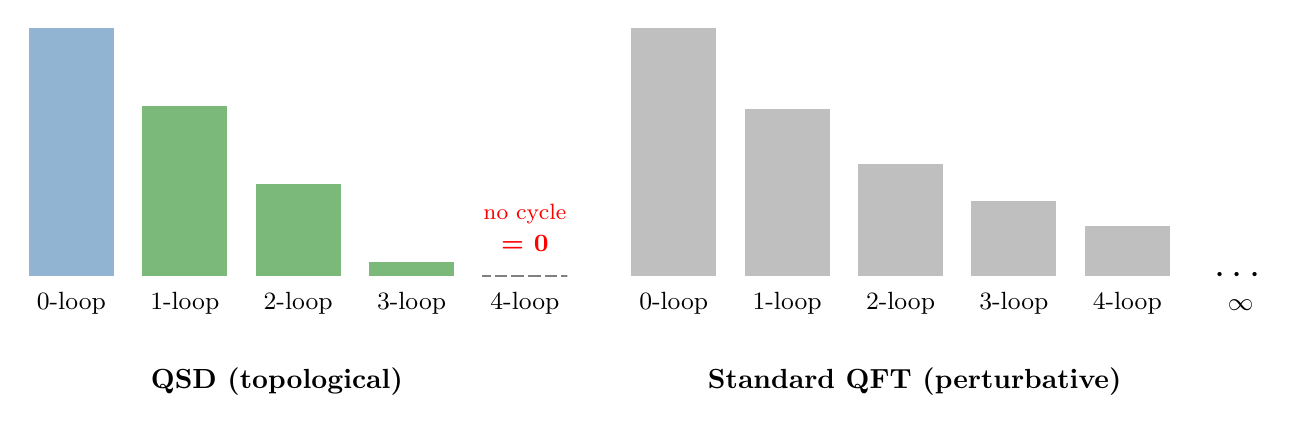
\begin{tikzpicture}[scale=0.9]
    % QSD: finite
    \begin{scope}[shift={(0,0)}]
        \node[font=\bfseries] at (3.5,-1.5) {QSD (topological)};
        \foreach \k in {0,1,2,3} {
            \pgfmathsetmacro{\h}{max(3.5-\k*1.1, 0)}
            \pgfmathsetmacro{\col}{ifthenelse(\k==0, "bulkcolor", ifthenelse(\k<4, "loopgreen", "gray"))}
            \fill[\col!60] (\k*1.6, 0) rectangle (\k*1.6+1.2, \h);
            \node[below, font=\small] at (\k*1.6+0.6, -0.1) {\k-loop};
        }
        % 4-loop: zero
        \draw[thick, dashed, gray] (4*1.6, 0) rectangle (4*1.6+1.2, 0);
        \node[below, font=\small] at (4*1.6+0.6, -0.1) {4-loop};
        \node[above, font=\small, red] at (4*1.6+0.6, 0.2) {\textbf{= 0}};
        \node[above, font=\footnotesize, red] at (4*1.6+0.6, 0.6) {no cycle};
    \end{scope}

    % QFT: infinite
    \begin{scope}[shift={(8.5,0)}]
        \node[font=\bfseries] at (4,-1.5) {Standard QFT (perturbative)};
        \foreach \k in {0,1,2,3,4} {
            \pgfmathsetmacro{\h}{3.5*exp(-0.4*\k)}
            \fill[gray!50] (\k*1.6, 0) rectangle (\k*1.6+1.2, \h);
            \node[below, font=\small] at (\k*1.6+0.6, -0.1) {\k-loop};
        }
        % Ellipsis
        \node[font=\Large] at (5*1.6+0.6, 0) {$\cdots$};
        \node[below, font=\small] at (5*1.6+0.6, -0.2) {$\infty$};
    \end{scope}
\end{tikzpicture}
\caption{Comparison: QSD terminates at 3 loops (topological constraint, 4-loop identically zero), while standard QFT has an infinite perturbation series~\cite{Wilson1974, Kinoshita2006} (each term smaller but never zero). The topological truncation is exact, not perturbative.}
\label{fig:qsd_vs_qft}
\end{figure}

This is the fundamental difference from standard QFT: the topology of the code structure \emph{truncates} the perturbation series. The truncation is topological (exact), not perturbative (approximate). This is analogous to modular invariance in string theory \cite{Polchinski1998v1}, though the mechanism here is combinatorial rather than geometric.

%==============================================================================
\section{Why Only $\alpha^{-1}$ Needs Loop Corrections}
\label{sec:why_only_alpha}
%==============================================================================

A natural question arises: if all three gauge couplings derive from the same building blocks, why does only $\alpha^{-1}_{\text{em}}$ require a loop series while $\alpha_s$ and $\sin^2\theta_W$ are accurate at tree level?

The answer is structural. The three observables access the $K_4$ graph in fundamentally different ways:

\begin{figure}[h]
\centering
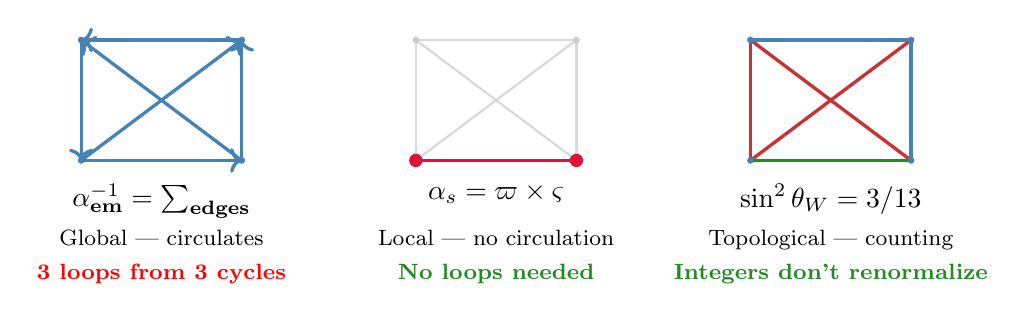
\begin{tikzpicture}[scale=0.85,
    obsbox/.style={draw, rounded corners, minimum width=3.4cm, minimum height=1.4cm, font=\small, align=center}]

    % α_em: global sum
    \begin{scope}[shift={(0,0)}]
        \coordinate (A) at (-1.2,-0.8);
        \coordinate (B) at (1.2,-0.8);
        \coordinate (C) at (1.2,1.0);
        \coordinate (D) at (-1.2,1.0);
        \foreach \i/\j in {A/B, B/C, C/D, D/A, A/C, B/D} {
            \draw[very thick, bulkcolor, ->] (\i) -- (\j);
        }
        \foreach \p in {A,B,C,D} {\fill[bulkcolor] (\p) circle (0.05);}
        \node[below, font=\normalsize\bfseries] at (0,-1.0) {$\alpha^{-1}_{\text{em}} = \sum_{\text{edges}}$};
        \node[below, font=\footnotesize] at (0,-1.7) {Global --- circulates};
        \node[below, font=\footnotesize, red] at (0,-2.2) {\textbf{3 loops from 3 cycles}};
    \end{scope}

    % α_s: local product
    \begin{scope}[shift={(5,0)}]
        \coordinate (A) at (-1.2,-0.8);
        \coordinate (B) at (1.2,-0.8);
        \coordinate (C) at (1.2,1.0);
        \coordinate (D) at (-1.2,1.0);
        \foreach \i/\j in {A/B, B/C, C/D, D/A, A/C, B/D} {
            \draw[thick, gray!30] (\i) -- (\j);
        }
        \foreach \p in {A,B,C,D} {\fill[gray!40] (\p) circle (0.05);}
        % Highlight single interaction
        \fill[anchorcolor] (A) circle (0.1);
        \fill[anchorcolor] (B) circle (0.1);
        \draw[very thick, anchorcolor] (A) -- (B);
        \node[below, font=\normalsize\bfseries] at (0,-1.0) {$\alpha_s = \varpi \times \gs$};
        \node[below, font=\footnotesize] at (0,-1.7) {Local --- no circulation};
        \node[below, font=\footnotesize, loopgreen] at (0,-2.2) {\textbf{No loops needed}};
    \end{scope}

    % sin²θ: counting
    \begin{scope}[shift={(10,0)}]
        \coordinate (A) at (-1.2,-0.8);
        \coordinate (B) at (1.2,-0.8);
        \coordinate (C) at (1.2,1.0);
        \coordinate (D) at (-1.2,1.0);
        % Group edges by gauge sector
        \draw[very thick, su3color] (D) -- (A);
        \draw[very thick, su3color] (A) -- (C);
        \draw[very thick, su3color] (B) -- (D);
        \draw[very thick, su2color] (B) -- (C);
        \draw[very thick, su2color] (C) -- (D);
        \draw[very thick, u1color] (A) -- (B);
        \foreach \p in {A,B,C,D} {\fill[bulkcolor] (\p) circle (0.05);}
        \node[below, font=\normalsize\bfseries] at (0,-1.0) {$\sin^2\theta_W = 3/13$};
        \node[below, font=\footnotesize] at (0,-1.7) {Topological --- counting};
        \node[below, font=\footnotesize, loopgreen] at (0,-2.2) {\textbf{Integers don't renormalize}};
    \end{scope}
\end{tikzpicture}
\caption{Why only $\alpha^{-1}_{\text{em}}$ requires loop corrections. Left: $\alpha^{-1}$ sums over all 6 edges, creating circulation around cycles --- this is what generates loop corrections. Centre: $\alpha_s = \varpi\gs$ is a local product that does not involve summation around paths. Right: $\sin^2\theta_W = 3/13$ is an integer ratio of generator counts; integers are topological invariants that do not receive loop corrections. The $\gs/32$ shift to $\sin^2\theta_W$ is a Hilbert space perturbation, not a loop.}
\label{fig:why_only_alpha}
\end{figure}

\begin{itemize}[nosep]
    \item \textbf{$\alpha^{-1}_{\text{em}}$}: A \emph{sum} over all 6 edges ($\sum_e \varpi/\Hbfour$). Summation over a closed graph means information circulates around cycles. Circulation around the 3 independent $K_4$ cycles generates 3 loop corrections. This is the graph-theoretic analogue of vacuum polarisation in QED.

    \item \textbf{$\alpha_s$}: A \emph{product} of local quantities ($\varpi \times \gs$). No summation over edges means no circulation, hence no loops. Like measuring voltage at a node rather than integrating around a circuit.

    \item \textbf{$\sin^2\theta_W$}: A \emph{ratio} of integer counts ($3/13$). Integer topological invariants do not renormalize---$3$ stays $3$ and $13$ stays $13$. The correction $\gs/32$ is a spectral perturbation from the Hilbert space dimension $2^5 = 32$, not a loop.
\end{itemize}

This structural distinction is satisfying: it is precisely the observable that involves \emph{global} information flow (summing around closed paths) that generates a perturbation series. The observables that probe \emph{local} or \emph{topological} properties are protected from loop corrections.

%==============================================================================
% REFERENCES
%==============================================================================

\bibliographystyle{unsrt}
\bibliography{qsd_references}

\end{document}
